 \documentclass[compsoc]{IEEEtran}
%
% If IEEEtran.cls has not been installed into the LaTeX system files,
% manually specify the path to it like:
% \documentclass[journal]{../sty/IEEEtran}

% Some very useful LaTeX packages include:
% (uncomment the ones you want to load)

\usepackage{xr}
\usepackage{cprotect} % include verb in c aption
\usepackage[utf8]{inputenc}
\usepackage{amsmath}
\usepackage{amsfonts}
\usepackage{url}
\usepackage{cprotect}
\usepackage[english]{babel}
\usepackage{hyperref}
\usepackage{caption}
\usepackage{subcaption}
\usepackage{float}
\usepackage{graphicx}
\usepackage{placeins}
\usepackage{xfrac}
\usepackage{spverbatim}
\usepackage{csquotes}
\usepackage[outputdir=../]{minted}
\usepackage[a4paper, margin={2cm, 2.5cm}]{geometry}
\hypersetup{
    colorlinks=true,
    linkcolor=black,
    filecolor=magenta,
    urlcolor=cyan
    }
\newcommand\numberthis{\addtocounter{equation}{1}\tag{\theequation}}
\newcommand{\rom}[1]{\uppercase\expandafter{\romannumeral #1\relax}}

\newcommand\Tstrut{\rule{0pt}{2.6ex}}       % "top" strut
\newcommand\Bstrut{\rule[-0.9ex]{0pt}{0pt}} % "bottom" strut
\newcommand{\TBstrut}{\Tstrut\Bstrut} % top&bottom struts

\newtheorem{defin}{Definition}
\newenvironment{definition}
  {\vspace{2pt}\par\noindent\begin{minipage}{.485\textwidth}\hrulefill\begin{defin}}
  {\par\noindent\hrulefill\end{defin}\end{minipage}\vspace{1pt}}


\begin{document}

\title{Robustness of the European Train Network}

\author{
Matteo Bonacini% <-this % stops a space
}
%\markboth{Journal of \LaTeX\ Class Files,~Vol.~14, No.~8, August~2015}


\onecolumn
% make the title area
\maketitle
% As a general rule, do not put math, special symbols or citations
% in the abstract or keywords.
\begin{abstract}
In this work I investigate the robustness of the European train network, modeled using passenger route data from the Trainline online platform. Degree distribution analysis reveals a scale-free topology characterized by a degree distribution exponent of $\gamma = 2.23$, placing the network within the ultra-small world regime. This configuration supports high resilience to random failures, with connectivity preserved even when up to $95\%$ of nodes are removed. However, the scale-free nature of the network also indicates vulnerability to targeted attacks: simulations show that removing just $20\%$ of the highest-degree nodes can
lead to network fragmentation. 
Community detection reveals the existence of four major communities which are locally more robust to targeted attacks and contribute to delay the effective destruction of the network. These findings highlight critical strengths and weaknesses within the European train network and suggest that more insight could be obtained by performing further studies.
\end{abstract}

\tableofcontents
\clearpage
\raggedbottom

\twocolumn

\section{Introduction}
The resilience and efficiency of transportation networks are critical to societal infrastructure, especially in interconnected systems like the European railway network, which facilitates daily commuting, economic trade, and tourism.

In this work, first I will construct a model by using the passenger train data available on the online platform \emph{Trainline}. The resulting network can be thought of as the network of all the train routes that European train companies serve. Even though its nature is different from the real-world railway infrastructure network, studying its robustness can be proven useful nonetheless, as it could allow companies to identify possible areas of improvement in their train routes.

Then, by using this model, I will show how the network handles in case of failure of an arbitray number of its nodes. I will present both theoretical results and numerical simulations, and I will compare them with previous works on a similar network. In order to best introduce the theoretical results, I will 
explain some concepts regarding network degree distribution, small world and scale free networks, node degree correlation and community subdivision.

Finally, I will present a summary of the result obtained and give ideas for further research.

\section{Extracting railway network data}
Nowadays, most passenger train companies provide online platforms on which people can buy train tickets. These platforms usually contain sufficient data to reconstruct some form of the railway network:
\begin{itemize}
    \item train numbers,
    \item station names.
    \item train routes between stations.
    \item travel time from one station to the next.
    \item network delays and failures.
\end{itemize}

One important piece of data that is \emph{not} available to the public is the physical track layout and throughput.
This means that, if one were to use data from this source, the resulting network would be made up of \emph{train routes}, rather than actual \emph{railways}. Even if some results will be similar, one must not forget that the two are very distinct entities.
Train routes are managed by different companies; they can vary quiclky in time due to demand and cost requirements. Railways, on the other hand, are physical structures that cannot be altered, unless a significant investment of time and money is made.

\subsection{Trainline}
\emph{Trainline} is a UK-based train-ticket company. They define themselves as: \blockquote{We are Europe’s leading train and coach app. To put it simply, we are a one-stop-shop for train and coach travel. Every day, we gather routes, prices, and travel times from over 270 rail and coach operators in 40 countries, so that everyone can buy tickets quickly and save time, effort, and money.\footnote{\url{https://www.thetrainline.com/about-us}}}
What their company does, in essence, is gather all the data from the major European train companies and then sell it. 
As a matter of fact, when a person buys a ticket through their platform, a small commision gets paid to Trainline, as an exchange for the ticket availability data\footnote{\url{https://www.trainlinegroup.com/what-we-do/business-model/}}.
The sale of the data can also happen at a larger scale, through their private-access \emph{Global Travel API}\footnote{\url{https://www.thetrainline.com/solutions/api}}. 

\subsection{Scraping the data}
\subsubsection{Legal Issues}
I was not able to obtain access to the Trainline API, and thus I had to manually scrape their data from their website. This came with the advantage that it was completely free, but with the drawback that it is a legal gray area. Although at the moment of writing their Terms of Service\footnote{\url{https://web.archive.org/web/20240716112036/https://www.thetrainline.com/terms}} do not appear to explicitly prohibit scraping, I consider the study I made in the following sections to be valid only for my personal use (that is, for the purpose of taking the Complex Networks exam).

\subsubsection{The scraping process}
Trainline offers a portal that contains a list of all of the stations reached by their routes\footnote{\url{https://www.thetrainline.com/en/stations}}.
From this webpage, it is possible to extract a list containing the URL for each station page by looking at its source code. Once we have this list, we can start downloading each page individually.
From every station page we can then extract the information of the most relevant destinations that can be reached from that station.
This whole process is described in detail in \autoref{fig:scraping-process}.

\begin{figure}
    \centering
    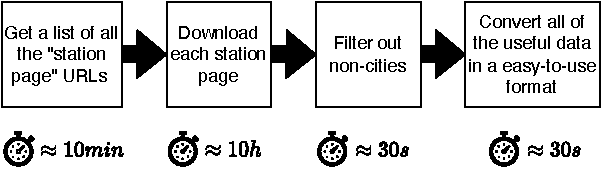
\includegraphics[width=1\linewidth]{report//assets/data-scraping.pdf}
    \cprotect\caption{Overview of the scraping process. The first step is getting a list of URLs for all of the train stations. This is done by hand, by analyzing the code of the \verb|/en/stations| page. The code contains one JavaScript array with the list of all URLs. With JavaScript it is easy to download each page programmatically. The maximum speed I was able to achieve was $\approx 20pages/s$, but that would trigger the CloudFlare DoS protection. In the end I had to let the scraper run overnight, with a speed of about one page every two seconds. The last step is just a matter of runinng through each HTML file with a RegExp that filters out all the needed data. This is pretty straighforward, as all the data is contained inside a JavaScript object which can be easily parsed. The third step is explained in the following section (\ref{subsubsec:data-in-numbers}).}
    \label{fig:scraping-process}
\end{figure}


\subsubsection{Data in numbers}
\label{subsubsec:data-in-numbers}
Before moving on, I want to point out again one subtlety in the data that I got. That is, Trainline offers information on two types of "station". Some are the \emph{real}, physical stations and some other are \emph{fictional aggregates} (which I will call \emph{cities}) of some number of real stations, usually found withing the same city.
This aggregate is generated by Trainline using some unknown algorithm. Even though I trust that this data is accurate, it might be difficult to track its source outside of Trainline.
For my study, I constructed the network using only the fictional aggregates.


Now, let us have a brief look at the data I got. 
In total, I have downloaded $18,502$ webpages ($4.95GB$ of data). Out of these, $248$ were cities. The total number of links reported between the cities was $1976$.


\subsection{Building the adjacency matrix}
Each station on the Trainline website has a list of the most common stations that can be reached starting from it. With this piece of information, it is easy to construct a (directed) adjacency matrix $A$. Moreover, the data contains the average number of trains per day that reach said destinations, and the average time it takes to get there. We can use this information to construct a rate matrix $W$ by multiplying each link by the ratio
\begin{equation*}
    \frac{\text{Number of daily trains through one route}}{\text{Average time it takes to complete the route}}.
\end{equation*}
The resulting matrix is plotted in \autoref{fig:asymm-plot-full} and a zoomed in, cropped version of it is plotted in \autoref{fig:asymm-plot-half}. The rows and columns have been sorted in order of population of the respective cities.
I find it nice to have a clear, human-readable plot of the (unweighted) data, and I provided it in \autoref{fig:big-plot}.

\begin{figure}[h]
    \centering
    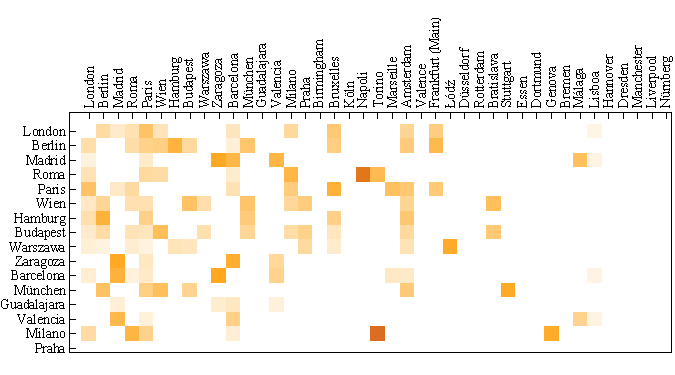
\includegraphics[width=\linewidth]{assets/asymmPlotHalf.pdf}
    \caption{
    Detail of the adjacency matrix of the European train network, sorted by city population. Dense connections are evident among major hubs (left side of the matrix), indicating high connectivity, but they decrease with smaller cities.}
    \label{fig:asymm-plot-half}
\end{figure}

The resulting matrix shows a gradient from left to right. This is a consequence of the fact that the Trainline data shows only the most common routes that start in any one city. It follows that
\begin{enumerate}
    \item smaller cities will often display link information to bigger cities (like country or state Capitals), and
    \item bigger cities will often display link information between themselves.
\end{enumerate}
In the zoomed-in graph of \autoref{fig:asymm-plot-half} it is easy to see this phenomenon: most links to the left of the matrix (where the big capital cities are) are two-ways and the matrix gets sparser and sparser the more we look to the right. 
This phenomenon indicates bias in the data, but it can easily corrected by making the assumption that \emph{every train that leaves a destination must come back to it}. We can then make the rate matrix symmetric by mirroring it across the diagonal\footnotemark. The resulting matrix is plotted in \autoref{fig:symm-plot}. 

\footnotetext{If a cell $W_{nm}$ is empty, and the transposed cell $W_{mn}$ is not, we set $W_{nm} = W_{mn}$. If both cells contain a value, we set each one of them to the average: $W_{nm} = W_{mn} = \frac 1 2 (W_{nm} + W_{mn})$.}


\section{Degree-distribution properties}
For each node $i$ in a undirected network, we can define its \emph{degree} $k_i$ as the number of edges connected to it. Formally, if $A$ is the adjacency matrix of the network, we define:
\begin{equation*}
    k_i = \sum_j A_{ij}.
\end{equation*}
Many useful properties of a network can be inferred by looking at its degree distribution.
In this section, we will show some of these properties, and how they apply to the Trainline network.

\subsection{Degree distribution}
There are two possible degree distributions that concern us:
\begin{enumerate}
    \item Poisson distribution and
    \item Power-law distribution.
\end{enumerate}

A network whose node degrees follow a power-law distribution is said to be a \emph{scale-free} network \cite{barabasi10}. Scale-free networks are prominent in nature and they exhibit some peculiar properties that we will briefly discuss below.
The Poisson distribution, on the other hand, is characteristic of random networks \cite{barabasi3, barabasi79} and it constitutes the null hypothesis.
If we were to find that the Trainline network followed a
Poisson degree distribution, it would probably mean that there is something wrong with the data.

The best way to look at the degree distribution is by plotting it on a double-logarithmic plot; if the data points show a linear behavior for several orders of magnitude, then it means that the network is scale-free\footnotemark. 
Given that the Trainline network has a relatively small number of nodes (for comparison, the WWW has over $300,000$ nodes \cite{barabasi9}, while the network I am using only has $248$), I have had some trouble in finding a fit  for the data points. The plot, the fit result(s) and the problems I encountered are all explained in \autoref{fig:degree-loglog}.
In the end, I concluded that the network shows a scale-free behavior $p(k) = C k^{-\gamma}$ with parameters $C=3.66$ and $\gamma=2.23$. These results are consistent with other results obtained in this paper and their meaning is discussed in the following chapter.

\footnotetext{A goodness-of-fit test would be in order to determine if the distribution is, in fact, a power-law.}


\begin{figure}[h]
    \centering
     \begin{subfigure}[h]{\linewidth}
         \centering
         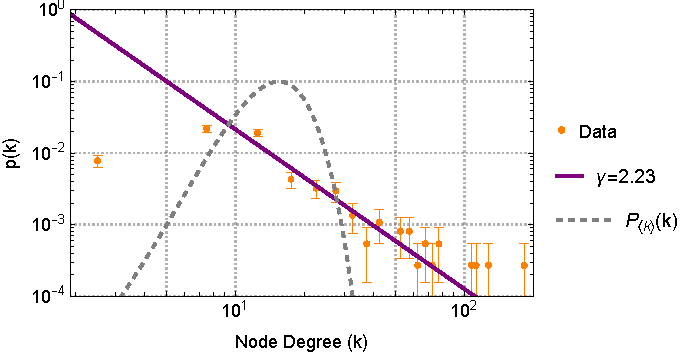
\includegraphics[width=\textwidth]{assets/degreePlotLinSpace.pdf}
         \caption{Data aggregation using linear binning. We show the best fit obtained by discarding the first two and last four points.}
         \label{fig:degree-logloglin}
     \end{subfigure}
     \hfill
     \begin{subfigure}[h]{\linewidth}
         \centering
         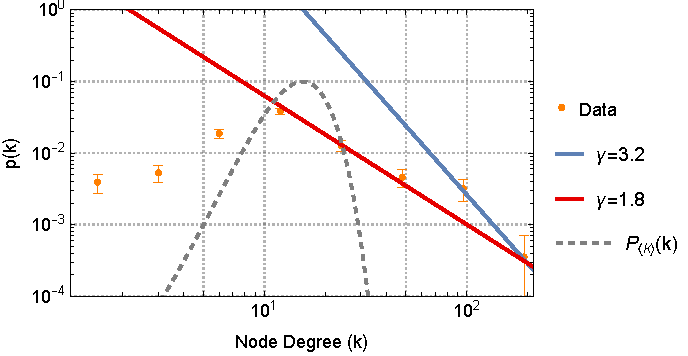
\includegraphics[width=\textwidth]{assets/degreePlotLogLog.pdf}
         \caption{Data aggregation using logarithic binning. Two possible fits are shown: one which takes into consideration only the last two points (blue) and one which takes into consideration the last five points (red). The latter has a value of $\gamma = 1.8$ which is anomalous (see section \ref{subsec:scale-free})   }
         \label{fig:degree-logloglog}
     \end{subfigure}
     \caption{Node degree distribution and fitting. The first plot (a) used linear binning to aggregate the data, while the second plot (b) used logarithmic binning. The results are different and, moreover, the values of $\gamma$ obtained in (b) are anomalous. When fitting these distribution, it is advised to use logarithmically-spaced bins; in this scenario, I believe the results which I obtained by using linearly-spaced bins are more reliable. In both plots, the dashed gray line is the best fit for a Poisson distribution (null hypothesis).  }
     \label{fig:degree-loglog}
\end{figure}


\subsection{Scale-free property}
\label{subsec:scale-free}
By definition \cite{barabasi}, a scale-free network is a network whose degree distribution follows a power law; that is:
\begin{equation}
    p(k) = C k^{-\gamma}.
    \label{eq:scale-law}
\end{equation}

In Nature we find that scale-free networks emerge in a wide variety of systems, such as: the internet \cite{barabasi99}, protein networks \cite{barabasi21}, metabolic networks \cite{barabasi20} and e-mail networks \cite{barabasi113}. The importance of scale-free networks arises from the fact that they exhibit some universal properties, that can be characterized solely by the exponent $\gamma$.
The main difference between a scale-free and a random network lies in the high-$k$ tail of the distribution. This difference is illustrated in \autoref{fig:degree-loglog}: here, we can see that the probability of finding a high-degree node in a scale-free networks is by orders of magnitude higher than in a random network. These high-degree nodes are often called \emph{hubs} and their existence plays a crucial role in determining both the robustness of a network and its small-world properties.
In \autoref{fig:degree-plot} I have shown how the node degrees are spatially distributed for the Trainline network. From this plot, it is easy to see that there are many, high-degree hubs spread troughout the whole network (they coincide with the busiest cities, as intuitively one would expect).

\begin{figure}[h]
    \centering
    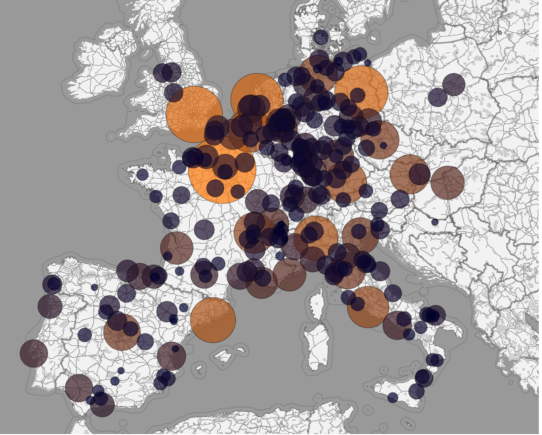
\includegraphics[width=1\linewidth]{report/assets/degreePlot.pdf}
    \caption{
    Visualization of the node degree distribution. The high-degree hubs correspond to European capitals and major cities. Each circle's color and size scale with the degree of its respective node.
}
    \label{fig:degree-plot}
\end{figure}

\subsubsection{Meaning of scale-free}
The origin of the term \emph{scale-free} comes from the fact that, for certain values of $\gamma$, the moments $\langle p(k)^n \rangle$ of the distribution \eqref{eq:scale-law} diverge if $n > 1$. Since the expectation value for a random variable $k$ exhibits fluctuations on the order of $\sqrt{\langle k^2 \rangle}$, having this value diverge would mean that, if we were to choose a node at random, we could expect it to be both arbitrarily small or large. This is in contrast to what we find for random networks, where the second moment is $\langle k^2 \rangle = \langle k \rangle^2$ and thus, the fluctuations are on the order of $\sqrt{\langle k \rangle}$. While in the latter case the average degree quantifies a scale for the fluctuations, in the former we cannot really define a scale due to the divergence of the second moment.

\subsubsection{(Ultra) small world properties}
\label{subsec:gammas}
Many of the properties of a scale-free network depend on the value of the exponent $\gamma$.
In this section, I will briefly discuss how $\gamma$ influences the \emph{small-world} property of a network; that is, the comparatively slower scaling of the average diameter $\langle d \rangle$ of a network with respect to its number of nodes. In other words, a network is said to exhibit small-world properties if the average distance between two nodes is relatively small, even if the number of nodes is very large. In the next sections, I will also show how the robustness properties of a scale-free network depend on $\gamma$.
A more in-depth explaination of these results can be found in \cite{barabasi}, and all of them can be obtained analytically \cite{barabasi120, barabasi121}.

\begin{itemize}
    \item $\gamma < 2$: \textbf{anomalous regime (\rom 1)}. Real, large networks cannot really follow this scaling law, as for $\gamma > 2$ we have that $\langle k \rangle$ diverges for large N. This would imply that the degree of the largest hub grows faster than the size of the network, which is not possible by definition.
    
    \item $\gamma = 2$: \textbf{anomalous regime (\rom 2)}. In this regime, we have that $\langle d \rangle \sim \text{constant}$. This means that the degree of the largest hub is approximately equal to the number of nodes in the network. This forces the network into a \emph{hub-and-spoke} configuration, in which all nodes are connected to a single, centralized hub.

    \item $2 < \gamma < 3$: \textbf{ultra-small world/scale free regime}. Here, we have that $\langle 
    d \rangle \sim \log{}\log N$; moreover, the first moment of $k$ converges, but all of the other moments diverge. In this regime, we find the presence of many high-degree hubs that are connected to small-degree nodes. This phenomenon effectively shrinks the distance between all the nodes of the network.

    \item $\gamma = 3$: \textbf{critical point}. Here $\langle d \rangle \sim \frac{\log N}{\log{} \log N}$, which is slower than the ultra-small wold regime but faster than the small-world regime.

    \item $\gamma > 3$: \textbf{small world/random network regime}. Here, $\langle d \rangle \sim \log N$ and $\langle k^2 \rangle$ converges. Hubs continue to exist, but they are not sufficiently large to make a significant difference with respect to a random network of the same size.
\end{itemize}

\subsection{Discussion of the fit results}
The proportionality constant $C$ of \eqref{eq:scale-law} can be obtained by imposing the normalization condition:
\begin{equation*}
    \sum _{k=1}^{+\infty} p(k) = 1.
\end{equation*}
Node degrees can only assume discrete values but, if we consider the limit in which the number of nodes is large, we can switch to the continuum formalism and compute $C$ more easily:
\begin{equation}
    \begin{aligned}
        C &= \frac{1} {\int_{k_{\min}}^{+\infty} k^{-\gamma} dk} \\
          &= (\gamma -1) k_{\min} ^{\gamma-1},    
    \end{aligned}
    \label{eq:kmin}
\end{equation}
where $k_{\min}$ is the smallest degree for which we expect the power law \eqref{eq:scale-law} to hold. The values of $k_{\min}$ and $\gamma$ can then be found by performing a fit on the data; the proper methodology can be found on \cite{barabasi}.

By plugging the fit result obtained in the previous section into \eqref{eq:kmin}, we obtain the estimate: $k_{\min} = 2.42$ and $\gamma=2.23$, which corresponds to the ultra-small world regime discussed in section \ref{subsec:gammas}.
This result is exactly what we would expect to obtain from a good transport network: the ultra-small world property implies that any node (city) can be reached in a short time by any other node, even if the two nodes considered are small, scarcely-connected cities.
Moreover, if we compute the mean graph distance of the Trainline network we obtain $\langle d \rangle = 2.28$, which is comparable to $\log{} \log N = 1.70$, as discussed in section \ref{subsec:gammas}. Graphically, we can get an idea of how the ultra-small world effect comes into play by looking at \autoref{fig:betweenness-plot}. There, I have plotted the \emph{betweennes centrality} $g(v)$ of each node $v$, which is a property related to the number of shortest paths that pass through it:
\begin{equation*}
    g(v) = \sum_{i \neq v \neq j} \frac{\sigma_{ij}(v)}{\sigma_{ij}},
\end{equation*}
where $\sigma_{ij}(v)$ is the number of shortest paths from $i$ to $j$ that pass through $v$ and $\sigma_{ij}$ is the number of all shortest paths from $i$ to $j$.
The nodes with very high betweenness centrality represent the hubs which are responsible for shortening the distances across the network.

At least one previous work \cite{gamma4} has run the same analysis on a similar European train network \cite{woodcock}, but they obtained a different result of $\gamma = 4.11$. The discrepancy of these results most likely comes from the different natures of the networks considered.

\begin{figure}
    \centering
    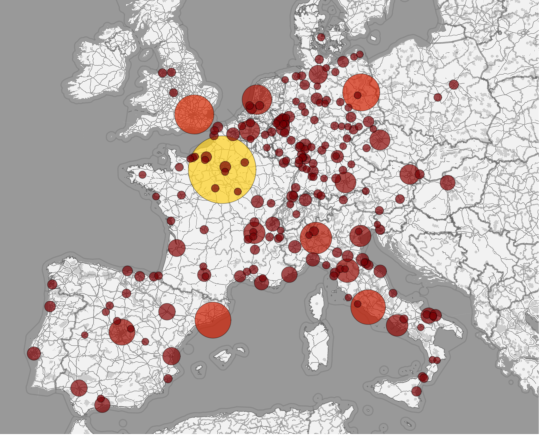
\includegraphics[width=1\linewidth]{report/assets/communitiesPlot.pdf}
    \caption{    Visualization of the node betweenness centrality distribution. The nodes with highest centrality correspond to European capitals and major cities. Each circle's color and size scale with the betweenness centrality of its respective node.}
    \label{fig:betweenness-plot}
\end{figure}

\section{Degree correlations}
Degree correlations quantify the likelihood of a high-degree node to connect to a low-degree node and vice-versa. They appear in many real-world networks (such as, the Internet, biological networks and social networks \cite{barabasi}), but not in all of them (e.g. the power grid does not exhibit degree correlations \cite{barabasi}). The study of degree correlation can help shed light on some network properties; 
for the scope of this work, what concerns us is the relation between degree correlations and network robustness.

\subsection{Possible cases}
We can distinguish three possible types of networks:
\begin{enumerate}
    \item \textbf{Neutral networks}. If there is no degree correlation, we say that a network is neutral. This is true, for example, in random networks.
    \item \textbf{Assortative networks}. This is the case if there is positive correlation between node degrees. In these types of networks, high-degree nodes tent to link to other high-degree nodes, and small-degree nodes to other small-degree nodes.
    \item \textbf{Disassortative networks}. This is the case if there is negative correlation between node degrees. Here, high-degree nodes tent to connect to low-degree nodes and vice-versa. 
\end{enumerate}

If the nodes of a network start randomly failing, we expect to see a phase transition at around some value of $\langle k \rangle$ for which the size of the giant component of the network falls to zero. Assortativity delays the phase transition in the following way:
\begin{itemize}
    \item In assortative networks, the phase transition happens at a lower value of $\langle k \rangle$, meaning that a higher number of nodes must fail in order to lose the giant component.
    \item In disassortative network, the opposite is true, meaning that the network will break up after a smaller number of nodes is removed.
\end{itemize}

\subsection{Measuring correlations}
Mathematically, all the information about degree correlation is contained in the \emph{degree correlation matrix} $e_{ij}$, which is defined as:
\begin{align*}
    e_{ij} = \text{Probability of finding nodes with degrees }\\ i \text{ and } j \text{ at the end of a randomly selected link.}
\end{align*}
One can compute \cite{barabasi} $e_{ij}$ explicitly for random networks. The result is:
\begin{equation*}
    e_{ij} = q_i q_j,
\end{equation*}
where $q_k$ is the probability of finding a node of degree-k at the end of a randomly selected link, given by
\begin{equation*}
    q_k = \frac{k\ p(k)} {\langle k \rangle}.
\end{equation*}
From an operative standpoint, working using $e_{ij}$ directly is quite cumbersome and thus, it is better to introduce the \emph{degree correlation function}:
\begin{equation*}
    k_{nn}(k) = \sum_{k'}k'P(k'|k).
\end{equation*}
$P(k'|k)$ is the probability to reach a degree-$k'$ node by following a link from a degree-$k$ node and thus $k_{nn}(k)$is the average degree of the neighbors of all degree-$k$ nodes.

The assortativity of a network depends on $k_{nn}(k)$ in the following way:
\begin{itemize}
    \item For neutral netowrks, we expect it to be a constant: $k_{nn}(k) = \langle k^2\rangle / \langle k\rangle$.
    \item For assortative networks, we expect it to follow a positive trend: $\frac d {dk} k_{nn}(k) > 0$.
    \item For disassortative networks, we expect the opposite: $\frac d {dk}k_{nn}(k) < 0$.
\end{itemize}

\subsection{Results from the data}
I have plotted the degree-correlation matrix in \autoref{fig:degree-corr-matrix} and, more importantly, the trend of the degree correlation function in \autoref{fig:corr-function}. From the latter, it is immediate to see that the data follows a downward trend; this means that the network is disassortative and thus more vulnerable to failures. Again, this result is not compatible with the one obtained in \cite{gamma4}, in which their network was observed to be assortative.

\begin{figure}[h]
    \centering
    \begin{subfigure}[h]{\linewidth}
        \centering
        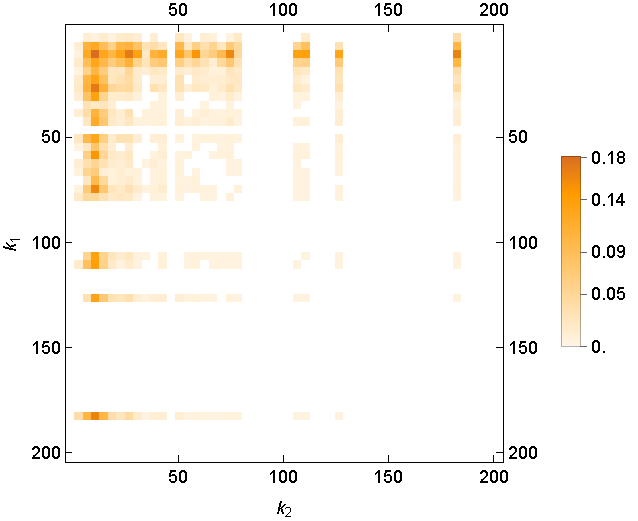
\includegraphics[width=.98\linewidth]{report/assets/assortativityMatrix.pdf}
        \caption{Degree correlation matrix}
        \label{fig:degree-corr-matrix}
    \end{subfigure}
    \hfill
    \begin{subfigure}[h]{\linewidth}
        \centering
        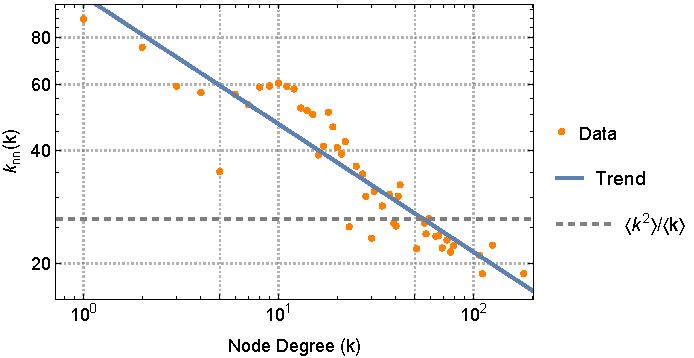
\includegraphics[width=1\linewidth]{report/assets/assortativityPlot.pdf}
        \caption{Trend for the degree correlation function. The fit indicates a downwards trend that follows the power law $\sim k^{-.34}$.}
        \label{fig:corr-function}
    \end{subfigure}
        \caption{Results of the degree correlation analysis: degree correlation matrix (a) and fit result for the degree correlation function (b).}
    \label{fig:assortativity}
\end{figure}
\section{Community subdivision}
Real-world network tend to be subdivided in many, smaller communities. This phenomenon is found in social networks \cite{barabasi283}, biological network \cite{barabasi288} and phone-call networks \cite{barabasi282}, and it has been of great interested for researchers since the early 2000s. One very good (and famous) example of the effect that the community subdivision can have on a network is the case known as \emph{Zachary's Karate Club} \cite{karateclub}. In this paper, the authors applied an autonomous community detection algorithm to the karate club participants' personal-interactions network which was able to predict the exact way in which the network fell apart after one major conflict struck the club.

This example illustrates how community detection can be a useful tool to quantify the robustness of a given network and to potentially predict its modes of failure under stress. In this chapter, I will briefly explain how communities can be defined and I will show how the Trainline network is subdivided.

\subsection{Defining communities}
Currently, there is not any widely-accepted definition of \emph{community}. Moreover, the mere existence of communities currently lacks any deep mathematical proofs and is based only upon empirical observations.  Barabasi \cite{barabasi} defines communities by using a series of hypotheses:
\begin{enumerate}
    \item Communities are structures uniquely encoded in a network's wiring diagram. The \emph{ground truth} of the community structure is to be discovered with algorithms.
    \item A community corresponds to a connected subgraph, whose connections are denser than with the rest of the network.
    \item Random networks do not have communities.
\end{enumerate}

Algorithms for community detection are constantly being developed \cite{communityDetection}; the main challenge for new algorithm is the difficulty in obtaining good results while maintaining a low computational complexity.
Given that the number of possible partition in a graph scales exponentially with its number of nodes \cite{barabasi}, a  simple brute-force approach would not work.

Currently, the best scaling algorithm is the Louvain method \cite{barabasi282}, which scales linearly with the number of links ($\mathcal O(L)$). There exist other algorithms that scale polinomially with the size of the network, up to the clique percolation algorithm \cite{cliquepercolation} which scales exponentially with the number of nodes ($\mathcal O(e^N)$). Ultimately, there does not exist a definitive \emph{best choice}; each algorithm has its own strength and weaknesses and should be used only within its intended use cases.

\subsection{Community detection results}
I have run a community detection algorithm on the Trainline network and the results are displayed in \autoref{fig:rainbow-plot}.
I have used the Mathematica function \verb|FindGraphCommunities| \cite{findgraphcommunities} with \verb|Methods->"Hierarchical"| settings. The official documentation does not state which exact algorithm the function implements, but it is most likely one of the hierarchical algorithms discussed in \cite{communityDetection}.

\begin{figure}
    \centering
    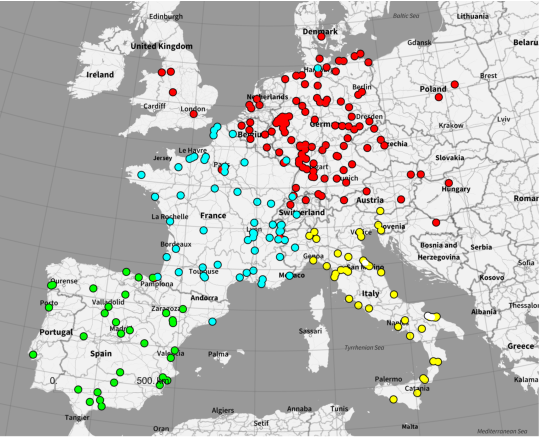
\includegraphics[width=1\linewidth]{report/assets/communitiesRainbow.pdf}
    \caption{Community structure of the Trainline network.
Four distinct communities are detected, roughly aligning with the geographic regions of Italy, France, Spain, and Germany. These regional clusters suggest that disruptions may cause localized isolation rather than complete network fragmentation.}
    \label{fig:rainbow-plot}
\end{figure}
Perhaps unsurprisingly, The algorithm managed to find four different communities which, for the most part, group the nodes which are situated in Italy, France, Spain and Germany. Given that, by definition, the link density is between community members is greater than with members of other communities, we can speculate that if the network were to face an attack, it would be less likely for a single community to immediately far apart, but more likely for different communities to remain isolated. 


\begin{figure}
    \centering
    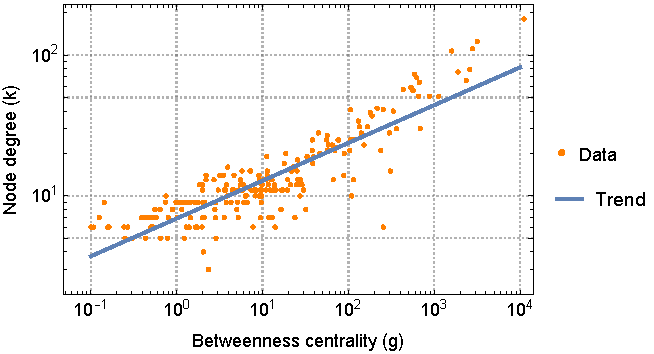
\includegraphics[width=1\linewidth]{report/assets/centralityDegreeCorrelation.pdf}
    \caption{Relationship between node degree and betweenness centrality.
    A positive correlation between the two is found, indicating that highly connected hubs also serve as primary paths in the network. This relationship shows how hubs are crucial in keeping the different communities connected together.}
    \label{fig:centrality-correlation}
\end{figure}
This is corroborated by the graph in \autoref{fig:centrality-correlation}, which shows that the degree of a certain node and its betweenness centrality are positively correlated. This, in turn, means that the more important a node is (i.e. the more links a certain city has), the higher is the number of shortest paths that pass through it. If an attack were to target the most important nodes first, it would make the travel time between nodes larger, up to infinity; if we assume that nodes in the same community are on average closer together, it is not unreasonable to assume that the shortest path between them will diverge slower than between nodes that are part of different communities.

The behavior of the network under an attack is discussed thoroughly in the next section.
\section{Network robustness}
The goal of studying network robustness is to see how a network behaves under some kind of failure. The most common form of failure that is studied is the removal of one node from a network. If the node is chosen at random, we call this a \emph{random failure} but if the node is chosen according to some heuristics, then we are talking about a \emph{targeted attack}. After the removal many properties of the network will change, but the one that concerns us the most is the probability $P_\infty$ with which a randomly selected node is part of the giant component.
In this section we will discuss some theoretical results and compare them with failure simulations on the Trainline network.

\subsection{Random failures}
When we gradually remove nodes from a network $P_\infty$ gets lower, up until it reaches zero. Under some condition, the network may undergo a phase transition and lead to $P_\infty$ reaching zero with a sharp drop, way before all of the nodes have been removed. This phase-transition behavior has been studied thoroughly within the framework offered by \emph{percolation theory} \cite{disorderedSystems}.
The results show that in a random network, the order parameter $P_\infty$ follows
\begin{equation*}
    P_\infty(f) \propto (f_c-f)^{\beta_f},
    \label{eq:percolation}
\end{equation*}
where $f$ is the fraction of nodes removed from the network, $f_c$ is a value dependent on the lattice type and $\beta_f$ is a \emph{critical exponent}. For reference, the value of $f_c$ for a two-dimensional square lattice is $f_c \approx .407$ and the value of $\beta_f$ is $\beta_f = 5/36$ (which is universal for lattices of dimension $2$).

When dealing with networks with an arbitrary degree distribution, however, we observe a different behavior. Relevant to us is the case of scale-free network, in which we do not see a sharp phase transition (for random failures, that is) but instead we find a steady, slow decline of $P_\infty$. Actually it can be proven that, for a network with an arbitrary degree distribution, we have a critical threshold $f_c$ on the fraction of nodes that we can remove, after which the network will completely lose its giant component. $f_c$ is given by \cite{barabasi16, molloyreed}:
\begin{equation}
    f_c = \ - \frac 1 {\frac {\langle k ^2 \rangle}{\langle k \rangle} - 1}.
    \label{eq:fc}
\end{equation}
Equation \eqref{eq:fc} predicts two different possible behaviors for scale-free network, depending on the value of $\gamma$:
\begin{itemize}
    \item For $\gamma < 3$, $\langle k^2 \rangle$ diverges and thus we get $f_c \to 1$ in the $N \to +\infty$ limit. This means that, in order to fragment the network, we need to remove all of its nodes.
    \item For $\gamma > 3$ we have that $f_c$ is independent of network size $N$, but depends only on $\gamma$ and $k_{\min}$. This behavior, proven in \cite{barabasi}, is the same as what we see in a random network: the network falls apart once a certain fraction of its nodes is removed.
\end{itemize}

I run a simulation on the Trainline network (\autoref{fig:random-failures}). Each data point in the plot is obtained by removing a certain fraction of nodes from the network and counting how many of the nodes are part of the giant component. This process is repeated $16$ times for each data point and the graph reports the standard deviation of all the results. The behavior we see is exactly what we expect from a scale free network with $\gamma < 3$. This result is great, as it indicates that the Trainline network is resilient to random failures of its node.
If, for example, a city were to be excluded from the network due to economical or environmental issues, the rest of the network would be able to keep working without any issues.

\begin{figure}[h]
    \centering
    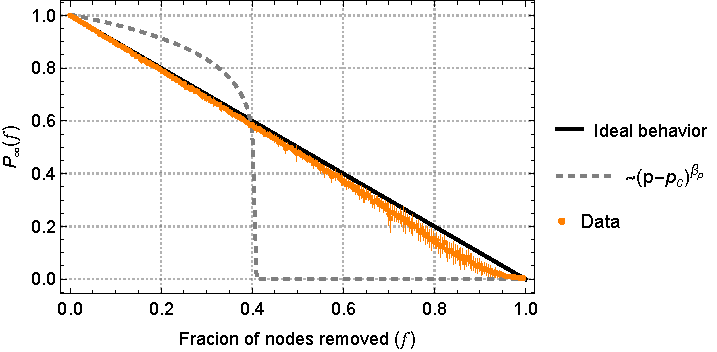
\includegraphics[width=1\linewidth]{report/assets/raindomFailuresPlot.pdf}
    \caption{Simulation of resilience of the network to random failures. Multiple runs were performed in which a certain number of nodes chosen at random was removed from the network. The graph shows the fraction of nodes that are still part of the giant component after the removal. The dashed, gray line is what we would expect to see if the network was wired like a 2-dimensional square lattice (null hypothesis).}
    \label{fig:random-failures}
\end{figure}


\subsection{Targeted attacks}
We have seen that scale free network are ideal if the mode of failure of the network is the removal of random nodes. What happens in the case of a targeted attack? 

\subsubsection{Attacking nodes}
We consider the case in which a potential attacker manages to disable the nodes in order of importance; that is, targeting the highest-degree node first. When this is the case, scale-free network do fail, and after only a small fraction of the nodes are removed \cite{barabasi12}.
It is possible to derive \cite{barabasi240} the following equation, whose solutions are the critical fraction of nodes that need to be removed by an attacker in order for the network to break apart completely:
\begin{equation}
    f_c^{\frac{2-\gamma }{1-\gamma }}= 2+ \frac{(2-\gamma )} {3-\gamma } k_{\min } \left(f_c^{\frac{3-\gamma }{1-\gamma }}-1\right).
    \label{eq:fc-attack}
\end{equation}
In our case, using the values of $k_{\min}$ and $\gamma$ that we obtained above, we get that $f_c = .235$ is the only acceptable solution. 

Again, we can confirm this behavior by running a simulation in which we remove the highest degree nodes, one at a time, and compute $P_\infty$ at each step.
The result (\autoref{fig:node-attack}) shows a fast, steady decline up to $f=.2$, after which we have a steep drop. At $f=.3$, more than $95\%$ of the network is now unreachable. This behavior matches what the theory predicts and highlights one very big weakness of the Trainline network.

\begin{figure}[h]
    \centering
    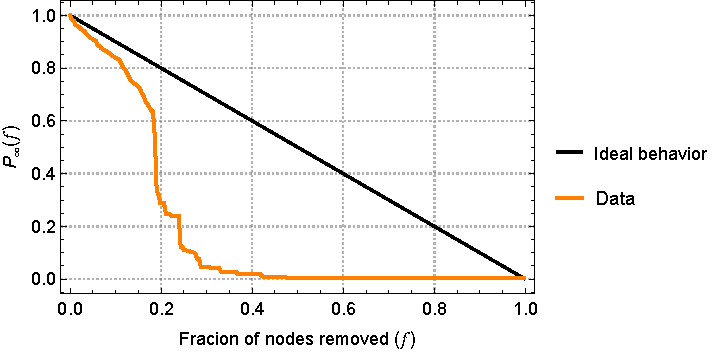
\includegraphics[width=1\linewidth]{report/assets/nodeAttackPlot.pdf}
    \caption{Simulation of resilience of the network to targeted attacks. One simulation was performed in which the highest-degree nodes were removed sequentially. The graph shows the fraction of nodes that are still part of the giant component after the removal.}
    \label{fig:node-attack}
\end{figure}

\subsubsection{Surviving communities}
We can make one interesting observation by plotting the community structure of the network just after the big drop at $f=.2$ (\autoref{fig:survivor-communities}). From this we can see that, even if the network is now fragmented, the individual communities more or less managed to survive. A network in this state would still be able to carry out some of its work; this means that the current attack strategy is a little less effective than what the calculations predict.

\begin{figure}[h]
    \centering
    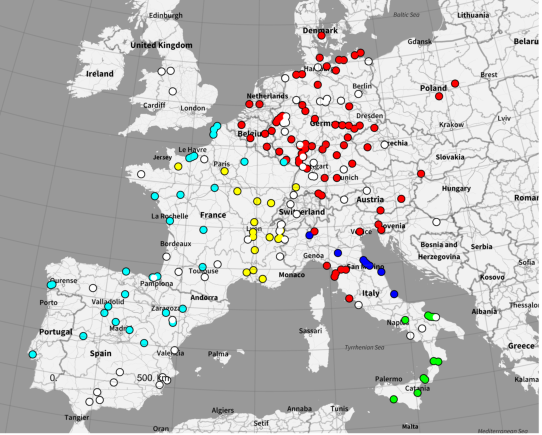
\includegraphics[width=1\linewidth]{report/assets/survivorCommunitiesVertexPlot.pdf}
    \caption{Survivor communities after the removal of the top $50$ highest-degree nodes. We can see that the community detection algorithm still manages to pick up some communities, meaning that some areas of the network manage to stay locally connected. The white dots group all the nodes that do not belong to any of the biggest communities.}
    \label{fig:survivor-communities}
\end{figure}


\begin{figure}[h!]
    \centering
    \begin{subfigure}[h]{\linewidth}
        \centering  
        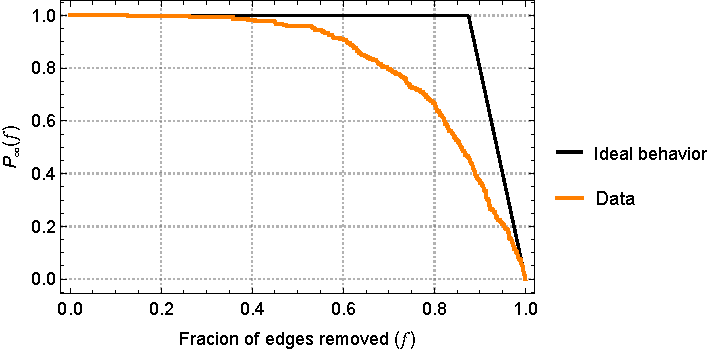
\includegraphics[width=\linewidth]{report/assets/edgeAttackGraph.pdf}
        \caption{Results of removing highest-througphut edges.}
        \label{fig:edge-attack-graph}
    \end{subfigure}
    \hfill
    \begin{subfigure}[h]{\linewidth}
        \centering
        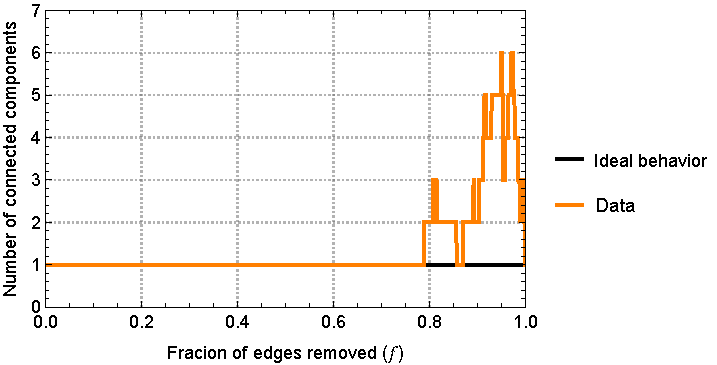
\includegraphics[width=.95\linewidth]{report/assets/edgeAttackComponentsPlot.pdf}
        \caption{Number of connected components after the highest-throughput edges are removed. The value of $1$ indicates that the whole network stays connected, up until the top $80\%$ of the edges are removed.}
        \label{fig:edge-attack-components}
    \end{subfigure}
    \caption{Simulation of resilience of the network to targeted edge attacks. One simulation was performed in which the highest-throughput edges were removed sequentially. The graph (a) shows the fraction of nodes that are still part of the giant component after the removal, while the graph (b) shows the number of components in which the network is split after the removal.}
    \label{fig:edge-attack}
\end{figure}


\subsubsection{Attacking edges}
To conclude this section I also wanted to explore how the network would behave if an attack were to be performed on the links, instead of on the nodes.
The rationale behind this is that train tracks, contrary to train stations, cannot be monitored throughout their whole length and thus could be more easily targeted by a destructive attack\footnotemark.

There is some research \cite{edgeremoval} on what is the best edge attack strategy, but it is mostly based on empirical results and lacks a deep theoretical study.
For my simulation, I chose the simplest attack strategy possible: remove the links according to their magnitude in the rate matrix $W$, starting from the highest to the lowest. The results (\autoref{fig:edge-attack}) show that the network is mostly untouched by this kind of attack. As a matter of fact, if we confront the two graphs in \autoref{fig:edge-attack-graph} and \autoref{fig:edge-attack-components} we can see that, even though $P_\infty$ starts to decay after $f=.4$, the number of connected components of the network stays constant throughout, up until $f=.8$.
This means that the removal of edges would, at most, only leave out singular nodes without fragmenting the network.

Given that edge attacks would be easier to execute, this result shows that the Trainline network might be more robust than what could transpire from the data in the previous section.



\footnotetext{Again, I would like to stress out that the Trainline network is very different from the European train track network. Nonetheless, in order for a link to exist on the Trainline network, there need to exist a physical track link as well.}


\subsection{Summary of the results}
Equations \eqref{eq:fc} and \eqref{eq:fc-attack} can be plotted together to show the predicted breakdown threshold of a scale-free network under the two possible moedes of failure. The result (\autoref{fig:fc-plot}) shows that for low values of $\gamma$, scale-free networks are susceptible to targeted attack and resilient to random failures. If the value of $\gamma$ gets too high, the value of $f_c$ tends to converge for both cases.

\begin{figure}[h]
    \centering
    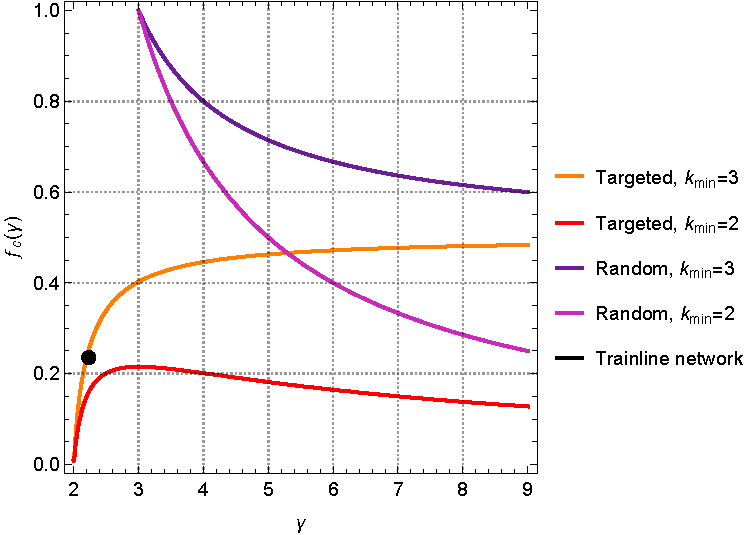
\includegraphics[width=1\linewidth]{report/assets/fcPlot.pdf}
    \caption{Plot of equations \eqref{eq:fc} and \eqref{eq:fc-attack}, which summarizes the resilience of a network as a function of the parameters $\gamma$ and $k_{\min}$. We can see that for low values of $\gamma$ a scale-free network is resilient to random failures but vulnerable to attacks. Over a certain threshold, the values fo $f_c$ tend to converge for both types of failures.}
    \label{fig:fc-plot}
\end{figure}

\section{Conclusions and future works}

\subsection{Conclusions}
In  this paper, we have shown how the Trainline network is scale-free. This fact alone dictates most of its robustness properties; mainly, we had predicted:
\begin{itemize}
    \item Very high tolerance to random node failures, and
    \item Low tolerance to targeted attacks.
\end{itemize}
The theoretical results matched perfectly the numerical simulations on the real-world data. We can summarise them with the following points.
\begin{itemize}
    \item The Trainline network is scale-free with degree exponent $\gamma=2.23$. It exhibits ultra-small world properties.
    \item If some number of randomly-chosen stations were to fail, the vast majority of all the other stations in the network would still be able to function normally.
    \item In the (unlikely) scenario in which the highest-degree stations were targeted by an attack, we would see the network fragment only after the top $20\%$ of nodes is taken out. Some large communities would still be standing up until the top $30\%$ of nodes is taken out.
    \item In the (more likely) scenario in which the highest-throughput links were targeted by an attack, the majority of the network would still be able to function normally, up until $80\%$ of the links are removed. Before that, only a few isolated stations would be cut off from the network.
\end{itemize}
My results differ from those obtained in \cite{gamma4}, but this might be due to the different nature of the networks considered.

\subsection{Future works}
This work highlighted some strengths and weaknesses of the Trainline network. While this network may be correlated with the physical train track network, in reality it is of a very different nature. The \emph{failing} of a node (or edge) in this network does not imply that the respective station has been shut off: it can also mean that one specific train company has decided to disable one of its routes due to economical reasons.
This robustness study is useful per se, but it might also be interesting to study the robustness properties of the \emph{physical} train tracks network, in which each link corresponds to some stretch of railroad. This network would allow multi-links and its properties could be different than those observed in this paper. This kind of study could help predict and prevent possible interruptions in the case of terrorist attacks or wars, for example.

Another possible line of work could be an analysis of the discrepancies between the results from this paper and the ones from \cite{gamma4}. Even though the network appears scale-free in both studies, the results in \cite{gamma4} suggest that the actual passenger transport network may be less robust than what the result in the present work suggest (due to a higher value of $\gamma$). A thorough study would need to compare different strategies for aggregating train timetable data into a network in order to find out which is the one that is most representative of the real world. Such network would probably contain both time-dependent links and multi-links.
%\clearpage

% \newpage 
\bibliographystyle{unsrt} % We choose the "plain" reference style
\bibliography{bibliography} % Entries are in the refs.bib file

\onecolumn
\clearpage
\appendices
\section{Large pictures}

\begin{figure}[h]
    \centering
     \begin{subfigure}[h]{.65\textwidth}
         \centering
         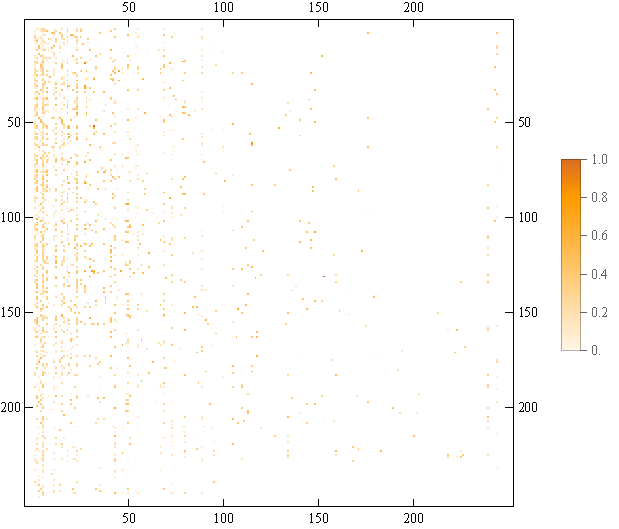
\includegraphics[width=\textwidth]{assets/asymmPlotFull.pdf}
         \caption{Original rate matrix}
         \label{fig:asymm-plot-full}
     \end{subfigure}
     \hfill
     \begin{subfigure}[h]{.65\textwidth}
         \centering
         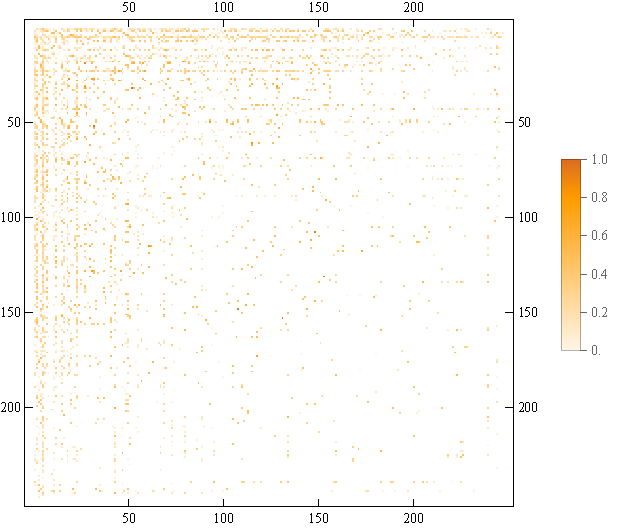
\includegraphics[width=\textwidth]{assets/symmPlotFull.pdf}
         \caption{Symmetrized rate matrix}
         \label{fig:symm-plot}
     \end{subfigure}
     \caption{Plot of the full, normalized rate matrix, sorted by city population.}
\end{figure}

\begin{figure}[b]
    \centering
    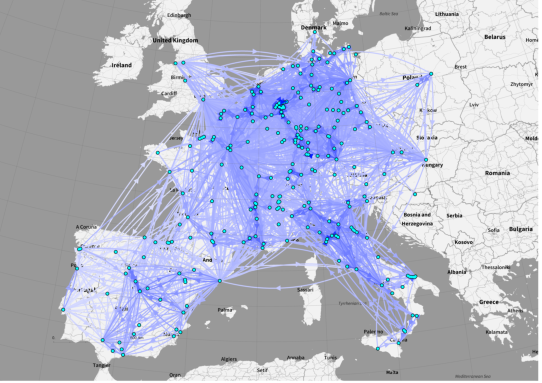
\includegraphics[angle=-90,origin=c,width=1\linewidth]{report/assets/rasterBigPlot.pdf}
    \caption{Big plot of the whole (unsymmetrized) network. The color of each arrow is proportional to its respective weight in the rate matrix $W$.}
    \label{fig:big-plot}
\end{figure}


\end{document}
